
\section{Aplicaciones de la Inteligencia Artificial en la Maquiladora,Inyección de Plásticos: Antes y Después del Machine Learning}

\subsection{Ranking de Adaptación}

\begin{table}[h!]
\centering
\caption{Ranking de Adaptación del Proyecto 1}
\resizebox{\textwidth}{!}{
\begin{tabular}{@{}>{\bfseries}l*{5}{>{\centering\arraybackslash}p{2cm}}@{}}
\toprule
Factor & Complejidad Técnica & Tiempo de Implementación & Inversión Económica & Capacitación del Personal & Impacto en la Cultura \\ \midrule
Valor & Alto (5) & Medio (3) & Alto (5) & Medio (3) & Alto (5) \\ \bottomrule
\end{tabular}}
\end{table}
\subsection{Por qué la Industria de Inyección de Plásticos es Ideal para Machine Learning}

La industria de inyección de plásticos, con su alto nivel de automatización y la necesidad constante de mejorar la eficiencia y la calidad, es un campo ideal para la implementación de \textbf{Machine Learning (ML)}. A continuación, se detallan las principales razones por las que esta industria puede beneficiarse enormemente de la adopción de ML:

\subsubsection{1. Abundancia de Datos}

Uno de los mayores desafíos en muchas industrias es la falta de datos consistentes y de calidad. Sin embargo, la industria de inyección de plásticos produce grandes volúmenes de datos que pueden aprovecharse para entrenar modelos de ML. Desde sensores en las máquinas que recopilan información sobre temperatura, presión, y tiempos de ciclo, hasta cámaras de visión por computadora que registran imágenes de cada producto, estos datos son fundamentales para:

\begin{itemize}
    \item Monitorear el rendimiento de las máquinas.
    \item Detectar defectos en tiempo real.
    \item Predecir posibles fallas mecánicas.
\end{itemize}

La abundancia de datos proporciona el material necesario para entrenar modelos de ML con un alto grado de precisión.

\subsubsection{2. Complejidad en los Procesos de Producción}

La inyección de plásticos involucra procesos que, aunque estandarizados, son complejos y tienen múltiples variables que afectan el resultado final. Entre estos se incluyen:

\begin{itemize}
    \item Variaciones en la temperatura del molde.
    \item Presión de inyección.
    \item Tiempo de enfriamiento.
    \item Calidad del material plástico.
\end{itemize}

El control manual o basado en reglas predeterminadas puede no ser lo suficientemente flexible para manejar todas estas variables de manera eficiente. Los modelos de ML, por otro lado, pueden analizar y aprender de grandes conjuntos de datos para optimizar automáticamente estos parámetros, mejorando tanto la calidad del producto como la eficiencia del proceso.

\subsubsection{3. Mejora en el Control de Calidad}

El control de calidad es un aspecto crucial en la industria de inyección de plásticos. Con métodos tradicionales, los defectos pueden no detectarse hasta después de que se haya completado la producción, lo que puede generar costos elevados por reprocesamiento y desperdicio de material. Con Machine Learning, es posible:

\begin{itemize}
    \item Utilizar \textbf{visión por computadora} para inspeccionar cada pieza en tiempo real.
    \item Detectar defectos como burbujas, deformaciones, o grietas de manera más precisa y rápida que con la inspección manual.
    \item Mejorar el control de calidad mediante el uso de \textbf{Redes Neuronales Convolucionales (CNNs)}, que aprenden a identificar patrones complejos en los productos inyectados.
\end{itemize}

La capacidad de realizar inspecciones en tiempo real reduce significativamente los defectos y garantiza que solo los productos de alta calidad lleguen al mercado.

\subsubsection{4. Mantenimiento Predictivo}

Las máquinas de inyección de plásticos están en operación constante, y las fallas inesperadas pueden ser extremadamente costosas debido al tiempo de inactividad y la pérdida de producción. Machine Learning puede analizar los datos en tiempo real para identificar patrones que indiquen cuándo una máquina está en riesgo de falla. De esta manera, las empresas pueden:

\begin{itemize}
    \item Implementar programas de \textbf{mantenimiento predictivo}, donde las reparaciones se realicen solo cuando son necesarias, basadas en datos.
    \item Reducir el tiempo de inactividad no planificado, aumentando así la eficiencia operativa.
    \item Alargar la vida útil de las máquinas mediante la identificación temprana de problemas potenciales.
\end{itemize}

\subsubsection{5. Optimización del Flujo de Trabajo}

Además de mejorar el control de calidad y el mantenimiento, Machine Learning también puede optimizar el flujo de trabajo en una planta de inyección de plásticos. Los sistemas MES (Manufacturing Execution Systems) pueden integrarse con algoritmos de ML para analizar los datos de producción en tiempo real y hacer recomendaciones sobre:

\begin{itemize}
    \item Ajustes en la programación de producción para evitar cuellos de botella.
    \item La distribución óptima de recursos en la planta.
    \item Cambios en los parámetros de operación para maximizar la producción sin comprometer la calidad.
\end{itemize}

Esto no solo mejora la eficiencia, sino que también permite a las plantas reaccionar de manera proactiva ante cualquier interrupción en la producción.

\subsubsection{6. Reducción de Costos Operativos}

Finalmente, la implementación de Machine Learning en la industria de inyección de plásticos puede conducir a una \textbf{reducción significativa en los costos operativos}. Las mejoras en la eficiencia, el mantenimiento predictivo, y el control de calidad no solo aumentan la producción, sino que también minimizan el desperdicio de materiales y reducen los costos de energía.

En resumen, la industria de inyección de plásticos es un campo ideal para Machine Learning debido a la abundancia de datos, la complejidad de los procesos, la necesidad de un control de calidad más eficiente, y los beneficios en mantenimiento y optimización de los flujos de trabajo. Adoptar ML permite a las plantas ser más competitivas, productivas y eficientes en un mercado global cada vez más exigente.


\subsection{El Problema del Scrap en Máquinas sin Mantenimiento}

El scrap o desperdicio es uno de los problemas más costosos en la industria de inyección de plásticos. Ocurre cuando las máquinas, debido a la falta de mantenimiento adecuado, comienzan a producir piezas defectuosas que no cumplen con los estándares de calidad. Este problema es especialmente crítico porque el scrap no solo representa una pérdida directa de materiales, sino también de tiempo y recursos.

\subsubsection{Causas del Scrap por Falta de Mantenimiento}

La falta de mantenimiento adecuado en las máquinas de inyección de plásticos puede tener varias consecuencias que derivan en scrap. Algunas de las principales causas son:

\begin{itemize}
    \item \textbf{Desgaste de Componentes Críticos}: Piezas como boquillas, barriles y tornillos de las máquinas inyectoras, si no reciben mantenimiento o reemplazo oportuno, comienzan a desgastarse. Este desgaste afecta directamente la calidad del producto final.
    \item \textbf{Malos Parámetros de Inyección}: Con el tiempo, las variaciones de temperatura y presión en la máquina debido a componentes mal calibrados o desgastados pueden causar inyecciones inexactas.
    \item \textbf{Acumulación de Residuos}: Las máquinas sin limpieza regular acumulan residuos en las cavidades y canales del molde, lo que provoca defectos en las piezas.
\end{itemize}

El scrap generado por estas causas no solo afecta la eficiencia de la planta, sino que también genera costos adicionales en el reprocesamiento de material o en la pérdida total de las piezas fabricadas.

\begin{figure}[H]
\centering
\includegraphics[width=0.7\textwidth]{img/scrap.jpg}
\caption{Ejemplo de scrap en piezas de plástico defectuosas debido a una máquina sin mantenimiento adecuado.}
\label{fig:scrap_problem}
\end{figure}



\subsection{Impacto Económico del Scrap por Falta de Mantenimiento}

El impacto económico del scrap generado por máquinas sin mantenimiento es significativo. A continuación, se describen algunos de los principales efectos:

\subsubsection{1. Pérdida de Materiales}

Cada vez que una pieza defectuosa es fabricada, se pierde material, que generalmente no puede ser reutilizado sin ser reprocesado. Esto es especialmente problemático cuando se trabaja con plásticos técnicos de alto costo, como el policarbonato o el nylon reforzado.

\subsubsection{2. Tiempo de Producción Perdido}

El tiempo dedicado a producir piezas defectuosas es tiempo perdido en la planta. Esto afecta directamente la capacidad de producción y puede generar retrasos en los envíos o incluso incumplimientos en los plazos de entrega a los clientes.

\subsubsection{3. Aumento en los Costos Operativos}

El scrap también genera un aumento en los costos operativos. Los costos de energía, mano de obra y uso de maquinaria aumentan, ya que se requiere más tiempo y recursos para producir una cantidad aceptable de piezas. Además, cuando las máquinas sin mantenimiento se detienen para reparaciones, las paradas no planificadas aumentan significativamente los costos.

\begin{figure}[H]
\centering
\includegraphics[width=0.7\textwidth]{img/scrap_fx.png}
\caption{Gráfico que muestra el impacto económico del scrap en una planta de inyección de plásticos.}
\label{fig:scrap_impact}
\end{figure}


\subWsection{Soluciones Basadas en Machine Learning para Reducir el Scrap}

Dado el impacto económico y operativo del scrap, una de las soluciones más prometedoras es la implementación de sistemas de Machine Learning para monitorear el estado de las máquinas y predecir cuándo se necesitarán tareas de mantenimiento. Las principales ventajas incluyen:

\begin{itemize}
    \item \textbf{Mantenimiento Predictivo}: Al monitorear los datos en tiempo real, el ML puede predecir cuándo una máquina está en riesgo de generar scrap, programando el mantenimiento necesario antes de que se produzca una gran cantidad de desperdicio.
    \item \textbf{Optimización de Parámetros de Producción}: ML puede ajustar automáticamente los parámetros de inyección, como la temperatura y la presión, para mantener la calidad de las piezas fabricadas dentro de los estándares deseados.
    \item \textbf{Reducción de Paradas No Planificadas}: Con ML, es posible anticipar fallos en las máquinas y realizar el mantenimiento en horarios planificados, evitando paradas inesperadas que generan scrap.
\end{itemize}

\begin{figure}[H]
\centering
\includegraphics[width=0.7\textwidth]{img/ob_scrapt.jpg}
\caption{Detección de defectos planta de inyección de plásticos.}
\label{fig:scrap_impact}
\end{figure} 

\subsection{Control de Calidad Automatizado}

El \textbf{control de calidad automatizado} es otra aplicación clave en la maquila, utilizando IA para inspeccionar productos en la línea de producción de forma más eficiente.

\begin{table}[h!]
\centering
\caption{Tecnologías Clave en Control de Calidad Automatizado}
\resizebox{\textwidth}{!}{
\begin{tabular}{@{}>{\bfseries}l*{3}{>{\raggedright\arraybackslash}p{4cm}}@{}}
\toprule
Aplicación & Beneficios & Tecnologías Clave \\ \midrule
Control de Calidad Automatizado & Detección rápida y precisa de defectos & Cámaras de Visión por Computadora, Redes Neuronales Convolucionales, Software de Análisis de Imágenes \\ \bottomrule
\end{tabular}}
\end{table}

% Diagrama de Control de Calidad Automatizado
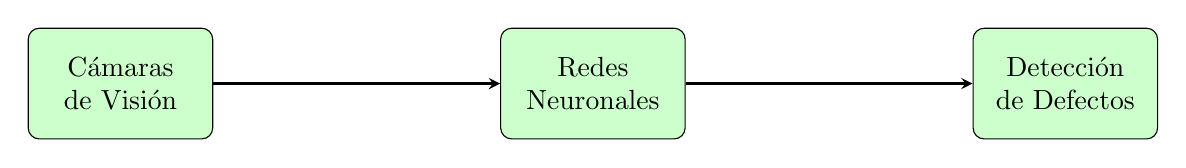
\begin{tikzpicture}[node distance=2cm]
\tikzstyle{block} = [rectangle, draw, fill=green!20, text width=6em, text centered, rounded corners, minimum height=4em]
\tikzstyle{arrow} = [thick,->,>=stealth]

\node (start) [block] {Cámaras de Visión};
\node (nn) [block, right of=start, xshift=4cm] {Redes Neuronales};
\node (quality) [block, right of=nn, xshift=4cm] {Detección de Defectos};

\draw [arrow] (start) -- (nn);
\draw [arrow] (nn) -- (quality);
\end{tikzpicture}

En el sector de la inyección de plásticos, el control de calidad automatizado es fundamental para garantizar que cada pieza cumpla con los estándares requeridos. Las cámaras de visión por computadora pueden identificar defectos como burbujas, deformaciones o imperfecciones en el moldeado.

\subsection{Optimización del Flujo de Trabajo}

La IA también puede ser utilizada para \textbf{optimizar el flujo de trabajo} en la maquila, analizando datos de producción y sugiriendo ajustes en tiempo real.

\begin{table}[h!]
\centering
\caption{Tecnologías Clave para la Optimización del Flujo de Trabajo}
\resizebox{\textwidth}{!}{
\begin{tabular}{@{}>{\bfseries}l*{3}{>{\raggedright\arraybackslash}p{4cm}}@{}}
\toprule
Aplicación & Beneficios & Tecnologías Clave \\ \midrule
Optimización del Flujo de Trabajo & Identificación de cuellos de botella, mejoras en la eficiencia & Sistemas MES, Análisis de Datos en Tiempo Real, Algoritmos de Optimización \\ \bottomrule
\end{tabular}}
\end{table}


% Diagrama de Optimización del Flujo de Trabajo
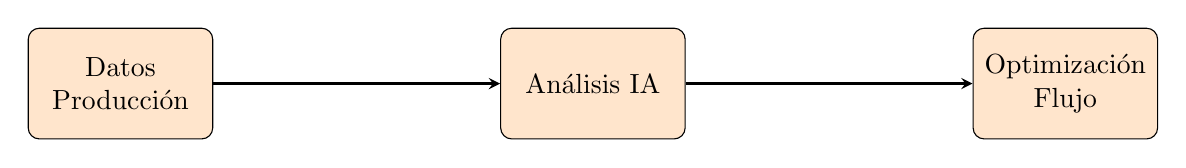
\begin{tikzpicture}[node distance=2cm]
\tikzstyle{block} = [rectangle, draw, fill=orange!20, text width=6em, text centered, rounded corners, minimum height=4em]
\tikzstyle{arrow} = [thick,->,>=stealth]

\node (start) [block] {Datos Producción};
\node (analysis) [block, right of=start, xshift=4cm] {Análisis IA};
\node (optimization) [block, right of=analysis, xshift=4cm] {Optimización Flujo};

\draw [arrow] (start) -- (analysis);
\draw [arrow] (analysis) -- (optimization);
\end{tikzpicture}

En el caso de una planta de inyección de plásticos, los sistemas MES como \textit{Siemens SIMATIC IT} pueden integrarse con la IA para detectar cuellos de botella en la producción. A través del análisis de datos en tiempo real, la planta puede ajustar la programación de los procesos, optimizando la utilización de las máquinas y reduciendo los tiempos muertos.

\subsection{Ejemplo en la Industria de Inyección de Plásticos}

En una planta de inyección de plásticos, la IA se puede aplicar de varias maneras para optimizar la operación:

\begin{enumerate}
    \item \textbf{Mantenimiento Predictivo}: Instalando sensores IoT en las máquinas de inyección, se puede monitorear el estado de las máquinas en tiempo real. La IA analiza los datos para predecir fallas, evitando costosas paradas de producción no planificadas.
    \item \textbf{Control de Calidad Automatizado}: Usando cámaras de visión por computadora y redes neuronales, la IA puede inspeccionar cada pieza de plástico en la línea de producción, detectando defectos en tiempo real.
    \item \textbf{Optimización del Flujo de Trabajo}: Con sistemas MES y análisis de datos en tiempo real, la IA puede ajustar dinámicamente el flujo de trabajo, evitando cuellos de botella y asegurando una producción continua y eficiente.
\end{enumerate}

Estas soluciones permiten que las plantas de inyección de plásticos aumenten su eficiencia, reduzcan los costos operativos y mejoren la calidad del producto final, lo que las hace más competitivas en el mercado global.

\subsection{Comparación Antes y Después del Machine Learning}

En esta sección, se muestra una comparación entre cómo se gestionaban distintos aspectos de la producción antes y después de la adopción de Machine Learning en la industria de inyección de plásticos. A través de esta comparación, se resaltan los beneficios clave que la IA ofrece.

\begin{table}[h!]
\centering
\caption{Antes y Después del Machine Learning en la Industria de Inyección de Plásticos}
\resizebox{\textwidth}{!}{
\begin{tabular}{@{}>{\bfseries}l*{2}{>{\raggedright\arraybackslash}p{6cm}}@{}}
\toprule
Proceso & Antes del Machine Learning & Después del Machine Learning \\ \midrule
Control de Calidad & Inspección manual, mayor probabilidad de error humano, identificación tardía de defectos. & Inspección automatizada en tiempo real con visión por computadora y redes neuronales, reduciendo errores y aumentando la precisión. \\ \midrule
Mantenimiento & Mantenimiento correctivo o basado en cronogramas predefinidos, alto costo por fallas inesperadas. & Mantenimiento predictivo utilizando sensores IoT y análisis de datos, anticipando fallas y reduciendo paradas no planificadas. \\ \midrule
Optimización del Flujo & Optimización reactiva basada en la experiencia del operador, identificación tardía de cuellos de botella. & Optimización proactiva del flujo de trabajo utilizando análisis de datos en tiempo real y algoritmos de Machine Learning. \\ \midrule
Eficiencia de la Producción & Dependiente de la habilidad del operador, con variabilidad en la calidad de los productos. & Eficiencia consistente y optimizada mediante el uso de algoritmos de optimización y ajustes automáticos en el flujo de trabajo. \\ \midrule
Toma de Decisiones & Basada en experiencia subjetiva, sin acceso inmediato a datos relevantes. & Toma de decisiones basada en datos, soportada por modelos predictivos que permiten mejorar la productividad y la calidad del producto. \\ \bottomrule
\end{tabular}}
}
\end{table}

\newpage

\subsection{Integración de Modelos de Lenguaje Grande (LLMs)}

Dada la creciente necesidad de optimización y automatización en la industria de inyección de plásticos, un paso inicial sencillo y efectivo para mejorar los procesos de producción es la integración de \textbf{Modelos de Lenguaje Grande (LLMs)} como primer paso, incluso si se obtiene una eficiencia inicial de solo el 61\%. 

Los LLMs pueden aportar beneficios significativos en la automatización de la comunicación interna, análisis de datos, y soporte en la toma de decisiones mediante interfaces de lenguaje natural.

\subsubsection{Eficiencia Inicial del 61\%}

Aunque la implementación de LLMs con una eficiencia inicial del 61\% puede parecer modesta, representa un avance significativo, ya que permite:

\begin{itemize}
    \item \textbf{Automatización de Consultas y Respuestas}: Los empleados pueden interactuar con el LLM para obtener respuestas rápidas sobre manuales técnicos, procedimientos de mantenimiento, y diagnósticos de fallas comunes, reduciendo el tiempo de búsqueda de información.
    \item \textbf{Soporte en la Toma de Decisiones}: El LLM puede asistir en la evaluación de datos históricos, sugiriendo posibles cursos de acción basados en patrones detectados en el historial de producción.
    \item \textbf{Mejora Gradual}: Con un punto de partida del 61\%, el sistema se puede ajustar y optimizar, alcanzando mayores niveles de eficiencia conforme se recopilan más datos y se refinan los modelos.
\end{itemize}

\subsection{Beneficios a Largo Plazo de los LLMs}

Los LLMs ofrecen una puerta de entrada para aumentar la eficiencia en la industria maquiladora, incluso con un nivel inicial de eficiencia limitado. Aquí algunos de los beneficios a largo plazo:

\begin{itemize}
    \item \textbf{Escalabilidad}: Una vez implementado, el modelo se puede entrenar con datos específicos de la planta, mejorando su precisión y alcance.
    \item \textbf{Reducción de Costos}: La automatización de tareas rutinarias y la mejora en la toma de decisiones reducirán los costos operativos a largo plazo.
    \item \textbf{Facilidad de Integración}: Los LLMs pueden integrarse fácilmente con los sistemas existentes, como ERPs y sistemas MES, para una mejor coordinación de los procesos productivos.
\end{itemize}

% Diagrama de Integración de LLMs
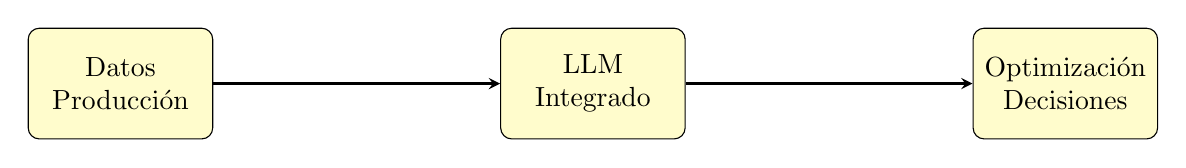
\begin{tikzpicture}[node distance=2cm]
\tikzstyle{block} = [rectangle, draw, fill=yellow!20, text width=6em, text centered, rounded corners, minimum height=4em]
\tikzstyle{arrow} = [thick,->,>=stealth]

\node (llm) [block] {LLM Integrado};
\node (data) [block, left of=llm, xshift=-4cm] {Datos Producción};
\node (output) [block, right of=llm, xshift=4cm] {Optimización Decisiones};

\draw [arrow] (data) -- (llm);
\draw [arrow] (llm) -- (output);
\end{tikzpicture}

En resumen, los LLMs pueden actuar como un primer paso accesible para automatizar y optimizar procesos en la maquiladora, con una eficiencia inicial del 61\%, que puede escalarse con el tiempo mediante ajustes y personalización del modelo.

\subsection{Conclusión}

La adopción de Machine Learning y la implementación de Modelos de Lenguaje Grande (LLMs) son pasos clave para transformar la industria de inyección de plásticos. Incluso con una eficiencia inicial del 61\%, los LLMs ofrecen una puerta de entrada hacia la automatización, la toma de decisiones basada en datos y la mejora continua, asegurando una ventaja competitiva a largo plazo.
